\section{Τεχνολογίες υλοποίησης} \label{subsection:4-3-implementation-technology-stack}

Η παρούσα ενότητα απαρτίζεται από υποενότητες, στις οποίες διατυπώνονται οι \textbf{σημαντικότερες} τεχνολογίες που χρησιμοποιήθηκαν για την υλοποίηση της εφαρμογής. Όλες οι τεχνολογίες αποτελούν δωρεάν λογισμικό ανοιχτού κώδικα.


\subsection{Τεχνολογίες σχετικές με το development}

Σε αυτήν την υποενότητα περιγράφονται ορισμένα θεμελιώδη εργαλεία και frameworks που συνετέλεσαν στην ανάπτυξη της εφαρμογής.

% TODO: add nodejs, docker, jenkins, janus and build steps diagram
4.3.1.development-technologies


\subsection{Τεχνολογίες σχετικές με το UI}

Στην παρούσα υποενότητα περιγράφονται όσες τεχνολογίες σχετίζονται με τη διεπαφή του χρήστη (UI), δηλαδή με το Presentation tier.

% TODO: add technologies like redux, sagas

\subsubsection{React} \label{subsection:4-3-2-1-react}

\logo{chapter-4/4.3.react-logo}{React logo}

Η React\footnote{\url{https://reactjs.org/}} αποτελεί βιβλιοθήκη Javascript, η οποία χρησιμοποιείται για την κατασκευή διεπαφών χρήστη. Είναι δηλωτική (declarative) και βασίζεται σε components, τα οποία διαχειρίζονται την κατάστασή τους (state) και συντίθενται για να δημιουργήσουν πολύπλοκα διαδραστικά UIs.

%TODO: When https://2021.stateofjs.com/en-US/ is available, add to the paragraph above that is the most popular js front-end framework (by usage), according to https://2020.stateofjs.com/en-US/technologies/front-end-frameworks/ and also add this beautiful chart.

Ένα σημαντικό εργαλείο για την ταχεία ανάπτυξη web εφαρμογών σε React είναι το Create React App\footnote{\url{https://create-react-app.dev/}}. Με τη χρήση μίας και μόνο εντολής (\texttt{npx create-react-app my-app}), εγκαθίσταται αυτόματα ένας development server σε περιβάλλον Node.js (ως μία μοναδική βιβλιοθήκη). Αυτός εμπεριέχει μία πληθώρα από build tools (π.χ. Webpack, Babel, ESLint), τα οποία προσφέρουν ισχυρές δυνατότητες, όπως άμεσα reloads και παραγωγή βελτιστοποιημένων bundles. Έτσι, η διαδικασία της υλοποίησης αποκτά ποικίλες διευκολύνσεις, χωρίς να απαιτεί την εκμάθηση, την χειροκίνητη εγκατάσταση και την προηγμένη διαμόρφωση των τεχνολογιών στο εσωτερικό. 

Η React έχει το αποθετήριό της στο GitHub (\url{https://github.com/facebook/react/}) και διατίθεται μέσω του μητρώου npm (\url{https://www.npmjs.com/package/react}).

\subsubsection{Redux} \label{subsection:4-3-2-1-redux}

\logo{chapter-4/4.3.redux-logo}{Redux logo}

Το Redux\footnote{\url{https://redux.js.org/}} αποτελεί μία βιβλιοθήκη Javascript, η χρήση της οποίας προσφέρει στην εφαρμογή ένα πλήρως διαχειρίσιμο κεντρικό state. 

%TODO: When https://2021.stateofjs.com/en-US/ is available, add to the paragraph above that is the most popular data layer technology (by usage), according to https://2020.stateofjs.com/en-US/technologies/datalayer/ and also add this beautiful chart.

Το Redux συνήθως χρησιμοποιείται για την κατασκευή διεπαφών χρήστη σε συνδύασμό με άλλες βιβλιοθήκες, όπως με την React. Σε αυτήν την περίπτωση, η λειτουργία του UI μπορεί να συνοψιστεί ως εξής:

%TODO: Add proper diagram
\begin{figure}[H]
	\centering
	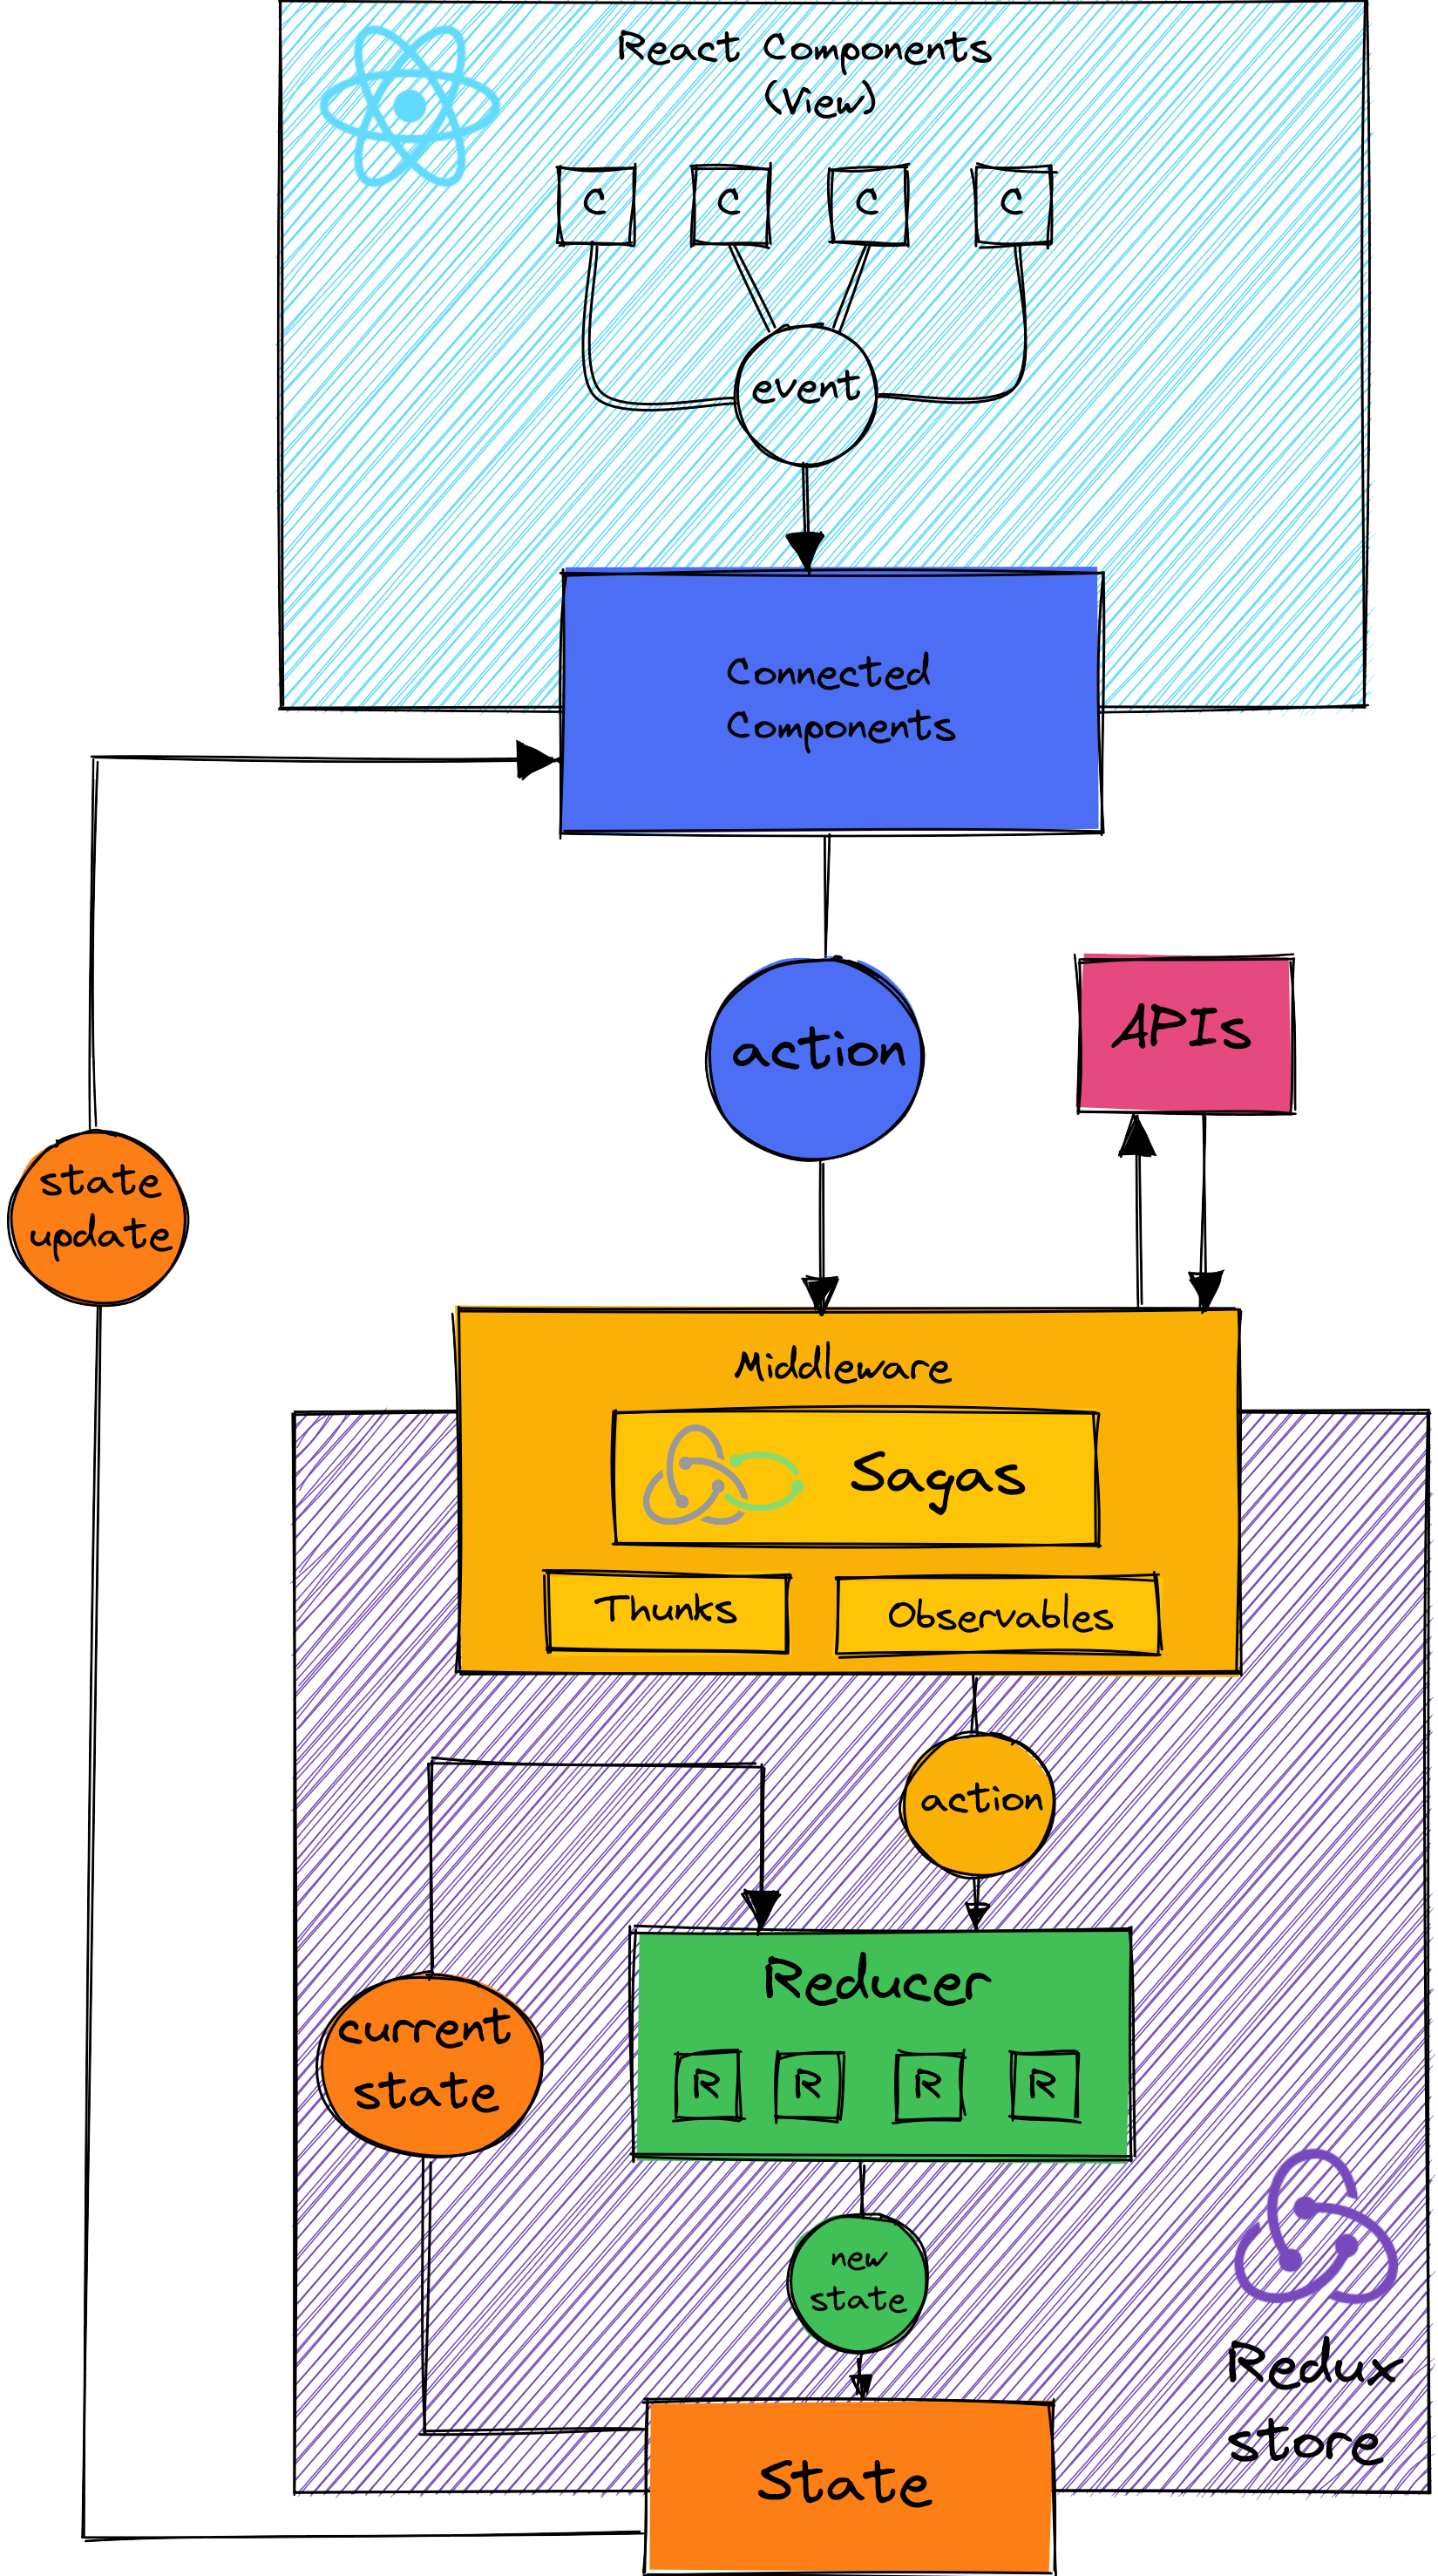
\includegraphics[width=.75\textwidth]{assets/figures/chapter-4/4.3.react-redux}
	\caption{Λειτουργία του Redux σε συνδυασμό με React}
\end{figure}

Το Redux έχει το αποθετήριό του στο GitHub (\url{https://github.com/reduxjs/redux}) και διατίθεται μέσω του μητρώου npm (\url{https://www.npmjs.com/package/redux}).

\subsubsection{Redux-Saga} \label{subsection:4-3-2-3-redux-saga}

\logo{chapter-4/4.3.redux-saga-logo}{Redux-Saga logo}

Το Redux-Saga\footnote{\url{https://redux.js.org/}} αποτελεί μία βιβλιοθήκη Javascript του οικοσυστήματος του Redux. Πρόκειται για ένα Redux middleware, το οποίο χρησιμοποιεί ESG generator functions\footnote{\url{https://developer.mozilla.org/en-US/docs/Web/JavaScript/Reference/Statements/function*}} για την εκτέλεση και διαχείριση ποικίλων ασύγχρονων side effect. Αυτές οι συναρτήσεις (sagas) παρέχουν μία πληθώρα επιλογών για την παράλληλη εκτέλεση κώδικα που μπορεί να σχετίζεται με εξωτερικά APIs, όπως με ένα blockchain ή μία βάση δεδομένων. Με αυτόν τον τρόπο, τα τελευταία μπορούν να συμπεριληφθούν στο κεντρικό Redux store και τη διαχείριση του συνολικού state της εφαρμογής.

Το Redux-Saga έχει το αποθετήριό του στο GitHub (\url{https://github.com/redux-saga/redux-saga}) και διατίθεται μέσω του μητρώου npm (\url{https://www.npmjs.com/package/redux-saga}).

\subsection{Τεχνολογίες σχετικές με το Ethereum} \label{subsection:4-3-3-ethereum-technologies}

Στην παρούσα υποενότητα περιγράφονται εκείνες οι τεχνολογίες που σχετίζονται με το Ethereum, δηλαδή με το Application tier της τεχνολογικής στοίβας.

\subsubsection{Truffle} \label{subsection:4-3-3-1-truffle}

\logo{chapter-4/4.3.truffle-logo}{Truffle logo}

Το Truffle\footnote{\url{https://trufflesuite.com/truffle/}} είναι ένα από τα δημοφιλέστερα Ethereum development frameworks και αποτελεί τμήμα της σουίτας Truffle.

Μέσω του Truffle πραγματοποιείται η διαχείριση των έξυπνων συμβολαίων. Αυτή περιλαμβάνει τη δοκιμή, τη σύνδεση και τη μεταγλώττισή τους, καθώς και την ανάπτυξη τους στο blockchain.

Επίσης, το Truffle περιέχει πρόσθετα σχετικά εργαλεία, όπως διαδραστική κονσόλα για άμεση αλληλεπίδραση με τα contracts  και εκτελεστής εξωτερικών σεναρίων (external script runner). 

Έχει το αποθετήριό του στο GitHub (\url{https://github.com/trufflesuite/truffle}) και διατίθεται μέσω του μητρώου npm (\url{https://www.npmjs.com/package/truffle}).
\subsubsection{Ganache} \label{subsection:4-3-3-2-ganache}

\logo{chapter-4/4.3.ganache-logo}{Ganache logo}

Το Ganache\footnote{\url{https://trufflesuite.com/ganache/}} είναι ένα λογισμικό που παρέχει ένα βοηθητικό προσωπικό Ethereum blockchain για ταχεία ανάπτυξη αποκεντρωμένων εφαρμογών και αποτελεί επίσης τμήμα της σουίτας Truffle. Διατίθεται τόσο ως desktop εφαρμογή με UI, όσο και ως CLI (command-line interface).

To Ganache παρέχει ισχυρά εργαλεία για την ανάπτυξη έξυπνων συμβολαίων, όπως:
\begin{itemize}
	\item Block explorer, μέσω του οποίου μπορούν να εξεταστούν λεπτομερώς όλα τα blocks και οι συναλλαγές που έλαβαν χώρα.
	\item Εξρεύνηση των εσωτερικών των contracts και των πυροδοτημένων event τους.
	\item Ενδελεχές αρχείο καταγραφής της εξόδου του blockchain, το οποίο περιλαμβάνει σημαντικές πληροφορίες για τον εντοπισμό σφαλμάτων.
	\item Δυνατότητα διαμόρφωσης του χρόνου εξόρυξης των block, έτσι ώστε να αρμόζει με τις εκάστοτε ανάγκες (αυτόματη εξόρυξη ή εξόρυξη σε προσαρμοσμένο χρονικό διάστημα).
\end{itemize}

\begin{figure}[H]
	\centering
	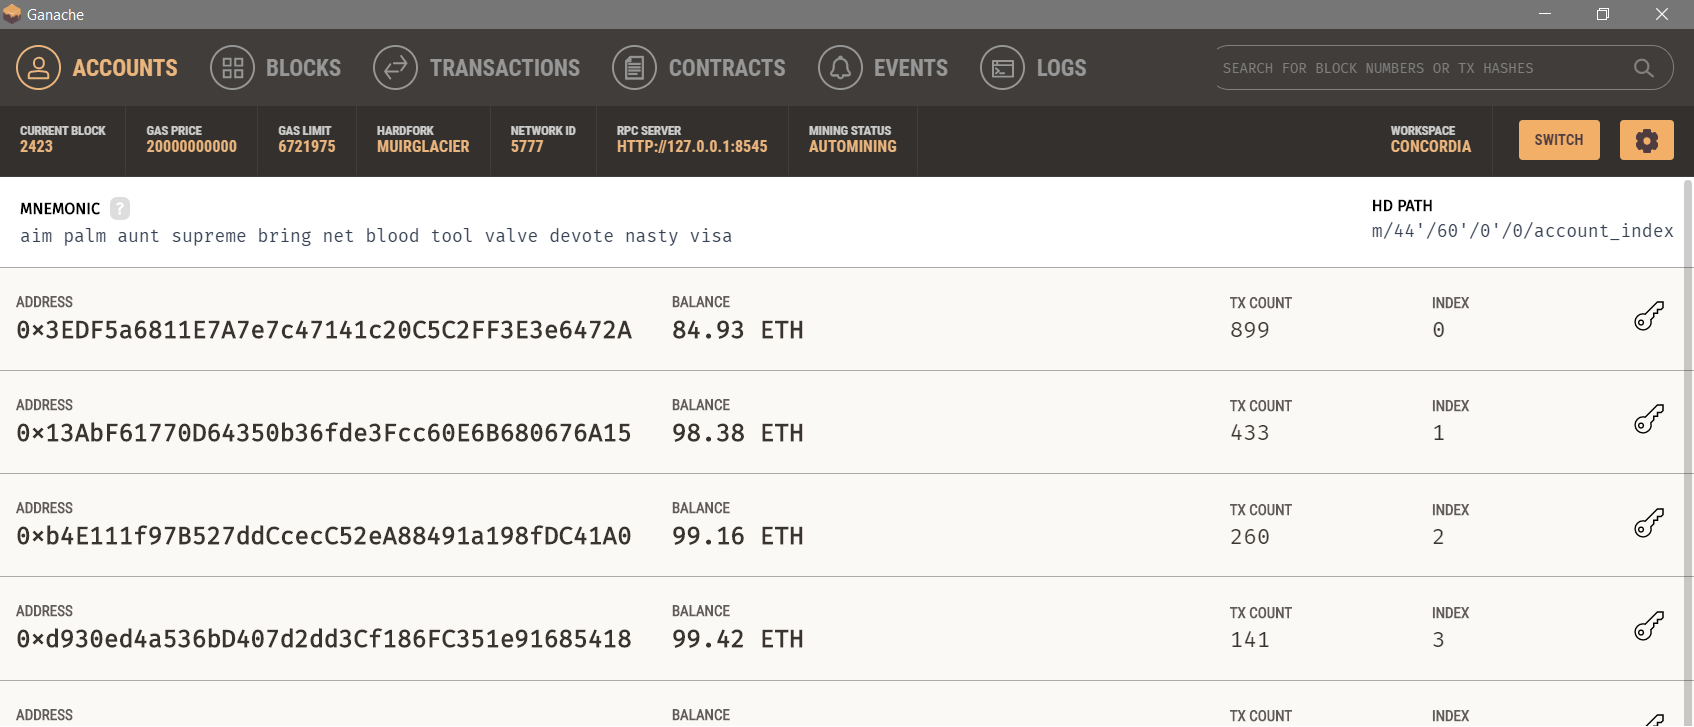
\includegraphics[width=.95\textwidth]{assets/figures/chapter-4/4.3.ganache-gui}
	\caption{Ganache (desktop εφαρμογή)}
\end{figure}

Το Ganache έχει το αποθετήριό του στο GitHub (\url{https://github.com/trufflesuite/ganache}) και διατίθεται μέσω του μητρώου npm (\url{https://www.npmjs.com/package/ganache}).

\subsection{Τεχνολογίες σχετικές με το IPFS}

Στην παρούσα υποενότητα θα περιγραφούν όσες τεχνολογίες σχετίζονται με το IPFS, δηλαδή με το Data tier.

\subsubsection{OrbitDB} \label{subsection:4-3-4-1-orbit-db}

\logo{chapter-4/4.3.orbitdb-logo}{OrbitDB logo}

Η OrbitDB είναι μία P2P βάση δεδομένων ανοιχτού κώδικα. Χρησιμοποιεί το IPFS για την αποθήκευση των δεδομένων και το IPFS Pubsub για τον αυτόματο συγχρονισμό των βάσεων δεδομένων μεταξύ των peers. Είναι τελικά συνεπής (eventually consistent) και χρησιμοποιεί CRDTs (Conflict-Free Replicated Data Types) για συγχωνεύσεις βάσεων δεδομένων χωρίς συγκρούσεις, πράγμα που την καθιστά εξαιρετική επιλογή για DApps και offline-first web applications.\cite{4.3-orbitdb}

Κάποια βασικά χαρακτηριστικά της είναι τα εξής:
\begin{itemize}
	\item \textbf{Stores}: Η OrbitDB παρέχει διάφορους τύπους βάσεων (stores) για διαφορετικά μοντέλα δεδομένων και περιπτώσεις χρήσης:
	
	\begin{itemize}
		\item log: ένα αμετάβλητο (μόνο για προσάρτηση) ημερολόγιο με ανιχνεύσιμο ιστορικό.
		\item feed: ένα μεταβλητό αρχείο καταγραφής με ανιχνεύσιμο ιστορικό, του οποίου οι καταχωρήσεις μπορούν να προστεθούν και να αφαιρεθούν.
		\item keyvalue: μία βάση δεδομένων κλειδιών-τιμών.
		\item docs: μία βάση δεδομένων εγγράφων στην οποία μπορούν να αρχειοθετηθούν έγγραφα JSON με ένα καθορισμένο κλειδί.
		\item counter: μία βάση δεδομένων για καταμέτρηση συμβάντων.
	\end{itemize}
	
	Όλα τα stores υλοποιούνται πάνω στο \texttt{ipfs-log}, μία αμετάβλητη, operation-based CRDT για κατανεμημένα συστήματα, ενώ υπάρχει και η δυνατότητα δημιουργίας προσαρμοσμένων stores ανάλογα με την περίπτωση.
	
	\item \textbf{Address}: Κάθε βάση δεδομένων λαμβάνει κατά τη δημιουργία της μία διεύθυνση της μορφής \texttt{/orbitdb/CID/DATABASE\_NAME}, όπου \texttt{CID} είναι το IPFS multihash του μανιφέστου της και \texttt{DATABASE\_NAME} το όνομα της βάσης.\cite{4.3-orbitdb-guide}Το μανιφέστο είναι ένα IPFS object που περιέχει πληροφορίες της βάσης όπως το όνομα, τον τύπο και έναν δείκτη στον ελεγκτή πρόσβασης (access controller).
	
	\item \textbf{Identity}: Κάθε φορά που προστίθεται μία εγγραφή στη βάση υπογράφεται από τον δημιουργό της, ο οποίος προσδιορίζεται από μία ταυτότητα (identity). Το Identity object, πέρα από τον προεπιλεγμένο τρόπο λειτουργίας, μπορεί να προσαρμοστεί έτσι ώστε να συνδέεται με κάποιο εξωτερικό αναγνωριστικό.
	Η μορφή του έχει ως εξής\footnote{Βλ. και \url{https://github.com/orbitdb/orbit-db-identity-provider}}:
	
	\begin{enumitemcenteredfigure}
		\simplelisting[width=.95\textwidth]{orbit-db-identity.js}
		\caption{OrbitDB Identity}
	\end{enumitemcenteredfigure}

	\item \textbf{Access Control}: Κατά τη δημιουργία μίας βάσης μπορούν να οριστούν όσοι θα έχουν δικαίωμα εγγραφής σε αυτή, μέσω ενός ελεγκτή πρόσβασης (access controller). Ο ελεγκτής θα περιλαμβάνει τα public keys τους, τα οποία μπορούν να ανακτηθούν από το identity του καθενός. Από προεπιλογή και αν δεν ορίζεται διαφορετικά, δίνεται πρόσβαση εγγραφής μόνο στον δημιουργό της βάσης.
\end{itemize}

Η OrbitDB έχει το αποθετήριό της στο GitHub (\url{https://github.com/orbitdb/orbit-db}) και διατίθεται ως μέσω του μητρώου npm (\url{https://www.npmjs.com/package/orbit-db}).

\subsubsection{Libp2p } \label{subsection:4-3-4-2-libp2p}

\logo{chapter-4/4.3.libp2p-logo}{Libp2p logo}

Η libp2p είναι ένα αρθρωτό σύστημα πρωτοκόλλων, προδιαγραφών και βιβλιοθηκών που επιτρέπουν την ανάπτυξη p2p εφαρμογών. Αποτελεί το υποκείμενο επίπεδο δικτύου του IPFS.\ref{2.7-ipfs-docs}

Ένα από τα υλοποιημένα πρωτόκολλα μεταφοράς δεδομένων της libp2p είναι το libp2p-webrtc-star\footnote{\url{https://github.com/libp2p/js-libp2p-webrtc-star}}. Αποτελεί το πρωτόκολλο μεταφοράς δεδομένων της εφαρμογής, καθώς υποστηρίζεται τόσο από Node.js servers, όσο και από browsers. Περιλαμβάνει, επίσης, έναν signalling server, που επιτρέπει τη γρήγορη διασύνδεση των peers.

Το libp2p-webrtc-star έχει το αποθετήριό του στο GitHub (\url{https://github.com/libp2p/js-libp2p-webrtc-star}) και διατίθεται μέσω του μητρώου npm (\url{https://www.npmjs.com/package/libp2p-webrtc-star}).


